\pdfminorversion=4\documentclass[hidelinks]{report}

\usepackage{graphicx}
\usepackage{times}
\usepackage{plain}
\usepackage[plainpages=false]{hyperref}
\usepackage{courier}
\usepackage{caption}

% To force figures to appear after text(along with [H] option)
\usepackage{float}

% To apply linespacing to some content
\usepackage{setspace}

% To show commands, code snippets
\usepackage{listings}

% To use checkmark (tick symbol)
\usepackage{amssymb}

\graphicspath{ {images/pdf/} }

\pagestyle{plain}

\fontfamily{Times}
\selectfont

\setlength{\textwidth}{6.5in}
\setlength{\textheight}{8.5in}
\setlength{\topmargin}{-0.25in}
\setlength{\oddsidemargin}{-0.00in}
\setlength{\evensidemargin}{-0.00in}

% To use multirow feature of latex tables
\usepackage{multirow}

% Using and defining own color
\usepackage{color}
\definecolor{mycol}{RGB}{52, 43, 41}

% Defining courier font usage syntax
\newcommand{\cf}[1] {
	\textbf{\texttt{#1}}
}

% Defining checkmark usage syntax
\newcommand{\T} {
	\checkmark
}

\begin{document}

%% Line spacing 1.5 applied
\setstretch{1.5}

\begin{center}
\section*{vEPC 1.0 User Manual}
\end{center}

\paragraph*{NOTE:}

The instructions given in this manual work only for linux-used machines, and might not work as expected on other OSes such as Mac and Windows. Please use online references in such cases. For details on understanding the code and various procedures involved in vEPC, please look at the \cf{developer\_manual.pdf} under \cf{doc} folder.

\subsection*{Installation}

\begin{enumerate}

\item Download vEPC repository, which includes \cf{doc}, \cf{scripts} and \cf{src} folders.

\item Navigate to \cf{scripts} folder and run \cf{install.h} file.

\begin{lstlisting}[language=bash]
$ bash install.h
\end{lstlisting}

This will install all the software modules/tools required for proper compilation and working of vEPC.

\item Navigate to \cf{src} folder and run \cf{makefile} to obtain binary executables for the individual software modules: MME, HSS, SGW, PGW, RAN, SINK.

\begin{lstlisting}[language=bash]
$ make
\end{lstlisting}

\item The following binary executable files would have been generated: \cf{mme.out}, \cf{hss.out}, \cf{sgw.out}, \cf{pgw.out}, \cf{ransim.out}, \cf{sink.out}. With these executables, you can now proceed to setup our vEPC, where individul modules will be hosted on separate Virtual Machines (VMs).

\end{enumerate}

\textbf{Note:} If there were any installation errors thrown by the compiler while running makefile, please install the corresponding dependencies. There should not be any other errors in this set of steps. Please note that the above procedure is provided only to understand the installation instructions, and it can be skipped to move directly to the Setup section.

\subsection*{Setup}

\begin{enumerate}

\item You will be requiring six VMs to setup our vEPC. Assign one VM for each software module (MME, HSS, SGW, PGW, RAN, SINK). Before proceeding, ensure proper communication among all VMs through the use of \cf{ping} command. Also, note down the \cf{eth0} IP addresses of VMs for future references.

\item Distribute the source code files into six sets according to the table~\ref{distribution} below. Eact set of \cf{.cpp/.h} files correspond to one of the EPC modules. Note that in table~\ref{distribution}, each file name (e.g., \cf{diameter}) corresponds to both \cf{.cpp} and \cf{.h} files (\cf{diamter.cpp} and \cf{diameter.h}).

\begin{table}[H]

\caption{Setup: Source code distribution.}
\centering
\label{distribution}
\def\arraystretch{1.5}

\begin{tabular}{|c|c|c|c|c|c|c|}

\hline
\textbf{MODULE} & \textbf{MME} & \textbf{HSS} & \textbf{SGW} & \textbf{PGW} & \textbf{RAN} & \textbf{SINK} \\
\hline
diameter & \T & \T & \T & \T & \T & \T \\
gtp & \T & \T & \T & \T & \T & \T \\
hss & & \T & & & & \\
hss\_server & & \T & & & & \\
mme & \T & & & & & \\
mme\_server & \T & & & & & \\
mysql & & \T & & & & \\
network & \T & \T & \T & \T & \T & \T \\
packet & \T & \T & \T & \T & \T & \T \\
pgw & & & & \T & & \\
pgw\_server & & & & \T & & \\
ran & & & & & \T & \\
ran\_simulator & & & & & \T & \\
s1ap & \T & \T & \T & \T & \T & \T \\
sctp\_client & \T & & & & \T & \\
sctp\_server & \T & \T & & & & \\
security & \T & & & & \T & \\
sgw & & & \T & & & \\
sgw\_server & & & \T & & & \\
sink & & & & & & \T \\
sink\_server & & & & & & \T \\
sync & \T & \T & \T & \T & \T & \\
telecom & \T & & & & \T & \\
tun & & & & & \T & \T \\
udp\_client & \T & & \T & \T & \T & \T \\
udp\_server & & & \T & \T & \T & \T \\
utils & \T & \T & \T & \T & \T & \T \\
\hline

\end{tabular}

\end{table}

\item Once source code files are segregated for each module (MME, HSS, SGW, PGW, RAN, SINK), place each set of files in its corresponding VM. Perform the following steps for each VM.

\begin{enumerate}

\item Open the main \cf{.cpp} file for the module (e.g., \cf{mme.cpp} for MME VM) and add the required IP addresses at the top of the file. For e.g., the set of IP addresses information required for SGW module is given below.

\begin{center}

\cf{string g\_sgw\_s11\_ip\_addr = "192.168.1.74";} \\
\cf{string g\_sgw\_s1\_ip\_addr = "192.168.1.74";} \\
\cf{string g\_sgw\_s5\_ip\_addr = "192.168.1.74";} \\

\end{center}

\item Copy the \cf{install.h} file from \cf{scripts} folder and run it to have all the required packages/tools in the VM. Install any additional tools that might be required (e.g., \cf{gedit, emacs})

\begin{lstlisting}[language=bash]
$ bash install.h
\end{lstlisting}

\item Copy the \cf{makefile} file from \cf{scripts} folder and run it for the corresponding module to have the updated binary executable.

\textbf{Sample run:}

\begin{lstlisting}[language=bash]
$ make mme.out
\end{lstlisting}

\end{enumerate}

\item \textbf{HSS:} Create MySQL database \cf{hss} in the VM assigned for HSS. 

\begin{lstlisting}[language=bash]
$ CREATE DATABASE hss
\end{lstlisting}

\item \textbf{HSS:} Copy the \cf{hss.sql} file from \cf{scripts} folder and run it to upload the necessary tables in MySQL database.

\begin{lstlisting}[language=bash]
$ mysql -p -u root hss < hss.sql
\end{lstlisting}

\end{enumerate}

The vEPC setup would be now complete and you can proceed to experimenting with our vEPC using different types of traffic. A sketch of the implemented setup is given in figure~\ref{setup}. Communication among modules will take place according to the dotted lines given in figure~\ref{setup}.

\begin{figure}[H]

\centering
\includegraphics[scale=0.4]{setup}
\caption{vEPC Setup.}
\label{setup}

\end{figure}

\subsection*{Generating Control traffic}

For experiments with control traffic, we simulate a number of concurrent UEs in the RAN simulator, and make the UEs continuously perform attach and detach procedures with the EPC, to create a continuous stream of control traffic. We increase or decrease load on the EPC by varying the number of concurrent UE threads loading the EPC. A detailed description of the procedure is given below.

\begin{enumerate}

\item Once the setup is ready, run each vEPC binary executable in its own VM. Usage format of each executable is given in table~\ref{bin_format} below. Please look at the \cf{developer\_manual.pdf} under \cf{doc} folder to understand more about the command line parameters used with each executable.

\begin{table}[H]

\caption{Usage format of binary executables.}
\centering
\label{bin_format}
\def\arraystretch{1.5}

\begin{tabular}{|c|p{11.5 cm}|}

\hline
\textbf{MODULE} & \textbf{USAGE} \\
\hline
MME & \cf{./mme.out <\#S1-MME threads>} \\
HSS & \cf{./hss.out <\#S6a threads>} \\
SGW & \cf{./sgw.out <\#S11 threads> <\#S1 threads> <\#S5 threads>} \\
PGW & \cf{./pgw.out <\#S5 threads> <\#SGi threads>} \\
\hline

\end{tabular}

\end{table}

A sample run of vEPC modules is given below.
~\\ \textbf{MME:}
\begin{lstlisting}[language=bash]
$ ./mme.out 50
\end{lstlisting}

\textbf{HSS:}
\begin{lstlisting}[language=bash]
$ ./hss.out 50
\end{lstlisting}

\textbf{SGW:}
\begin{lstlisting}[language=bash]
$ ./sgw.out 50 50 50
\end{lstlisting}

\textbf{PGW:}
\begin{lstlisting}[language=bash]
$ ./pgw 50 50
\end{lstlisting}

\item \textbf{RAN:} Open \cf{ran\_simulator.cpp} and comment out the following code sections.

\begin{itemize}

\item \cf{data\_transfer} section under the \cf{simulate} function.

\item \cf{tun} and \cf{traffic\_monitor} sections under the \cf{run} function.

\end{itemize}

By doing this, you are simulating \cf{RAN} objects that generate only control traffic.

\item \textbf{RAN:} Rerun the \cf{makefile} for the RAN module to make the binary executable for generating only control traffic.

\begin{lstlisting}[language=bash]
$ make ransim.out
\end{lstlisting}

\item \textbf{RAN:} Start RAN simulator with appropriate parameters as given below. This will generate the required amount of control traffic for the given time duration.

\begin{center}

\cf{./ransim.out <\#RAN threads> <Time duration>}

\end{center}

A sample run is as follows.

\begin{lstlisting}[language=bash]
$ ./ransim 10 100
\end{lstlisting}

\end{enumerate}


\subsection*{Generating Data traffic}

For experiments with data traffic, we attach a specified number of UEs to the EPC from the RAN simulator, and pump traffic from the RAN to the sink. A traffic generating tool called \cf{iperf3} is employed, using which TCP data can be sent with a given bandwidth and time duration. To generate traffic, \cf{iperf3} process is started in Server mode at the Sink module and the corresponding \cf{iperf3} Client process is started at the RAN simulator with the required input data rate and time duration parameters. A detailed description of the procedure is given below.

\begin{enumerate}

\item Begin vEPC modules (MME, HSS, SGW, PGW) as explained before.

\item \textbf{SINK:} Start the Sink module with the required number of \cf{iperf3} servers.

\begin{center}

\cf{./sink.out <\#iperf3 servers>}

\end{center}

A sample run is as follows.

\begin{lstlisting}[language=bash]
$ ./sink 10
\end{lstlisting}

\item \textbf{RAN:} Open \cf{ran\_simulator.cpp} and uncomment the following code sections: \cf{data\_transfer, tun, traffic\_monitor}. 

\item \textbf{RAN:} Open \cf{ran.cpp} and set the duration of \cf{iperf3} data transfer - \cf{dur} under the \cf{transfer\_data} function. Note that this duration has to be smaller than the overall duration given as command line parameter while running RAN simulator. Input data rate is currently fixed at 1 Mbps. It can be modified as per requirements.

\item \textbf{RAN:} Rerun the \cf{makefile} for the RAN module to reflect the updates in the binary executable.

\begin{lstlisting}[language=bash]
$ make ransim.out
\end{lstlisting}

\item \textbf{RAN:} Now begin the RAN simulator as explained before. This will simulate the required number of \cf{RAN} objects, generating both control traffic and data traffic in sequence, for the given time duration. Note that the number of \cf{RAN} objects created has to be equal or greater than the number of \cf{iperf3} servers started at Sink module.

\end{enumerate}

\subsection*{Performance results}

\paragraph*{Control traffic}

~\\ Two performance metrics would be reported at the end of control traffic experimentation. These parameters are given below. No additional scripts/coding would be required to produce these parameters as they are computed along with the generation of control traffic. 

\begin{enumerate}

\item \textbf{Throughput}, the number of registration requests successfully completed by the EPC per second

\item \textbf{Latency}, the time taken by a registration to complete

\end{enumerate}

\paragraph*{Data traffic}

~\\ While experimenting with data traffic, the following steps need to be followed to obtain performance results.

\begin{enumerate}

\item \textbf{SINK:} Copy the \cf{find\_bw.sh} file from \cf{scripts} folder. Just before starting the RAN simulator, run this script at the Sink module. This will measure the required throughput value. A file named \cf{bw.txt} will be created, which contains the various throughput values (in bytes/second): Uplink, Downlink, Total (Uplink + Downlink). 

\textbf{Format:}
\begin{center}

\cf{bash find\_bw.sh -i <interface> -s <duration> -c <count> -n <\#UEs>} 

\end{center}

\textbf{Sample run:}

\begin{lstlisting}[language=bash]
$ bash find_bw.sh -i eth0 -s 100 -c 1 -n 1
\end{lstlisting}

\item \textbf{RAN:} Before starting the RAN simulator, open \cf{ran\_simulator.cpp} and uncomment the \cf{RTT} code section under the \cf{simulate} function. This will create a \cf{ping.txt} file, which contains the Round Trip Time (RTT) latency values for the data transfer in milliseconds. Note that the time duration under \cf{ping} function need to be set according to the time duration of the user data transfer.

\end{enumerate}

With the procedure explained above, two performance metrics would be obtained at the end of data traffic experimentation. These parameters are given below.

\begin{enumerate}

\item \textbf{Throughput}, the amount of data traffic successfully forwarded by the EPC gateways to the Sink per second

\item \textbf{RTT Latency}, the amount of processing overhead added by the EPC gateways in the data
plane, as measured by a ping command during load test

\end{enumerate}

\end{document}